\documentclass[11pt]{article}

\usepackage{sectsty}
\usepackage{hyperref}
\usepackage{graphicx}
\usepackage{amsmath}
\usepackage{biblatex}
\usepackage{nicefrac}
\usepackage{float}
\usepackage{graphicx}    
\usepackage{subcaption}
\addbibresource{refs.bib}

% Margins
\topmargin=-0.45in
\evensidemargin=0in
\oddsidemargin=0in
\textwidth=6.5in
\textheight=9.0in
\headsep=0.25in

\hypersetup{
    colorlinks=true,
    linkcolor=blue,    % Color for internal links (e.g., table of contents)
    urlcolor=red,      % Color for external URLs
    citecolor=green    % Color for citations
}

\title{A short report on shape comparison metrics}
\author{Martin Metodiev}
\date{\today}

\begin{document}
\maketitle	


% Optional TOC
% \tableofcontents
% \pagebreak

%--Paper--

\section{Introduction}

Here we review some useful metrics for shape analysis. Ideally, a shape metric will be independent of the relative spatial location of two objects, and also rotational and scaling variations \cite{shapedna}, \cite{hyp_w}. An intuitive approach is to use the Hausdorff distance as a measure of similarity between two sets \( A \) and \( B \):

\begin{equation}
d_H(A, B) = \max \left( \sup_{a \in A} \inf_{b \in B} \| a - b \|, \sup_{b \in B} \inf_{a \in A} \| a - b \| \right)
\end{equation}


Unfortunately this approach does not take into account the connectivity of the mesh and only considers the vertices. This implies that physical information, such as roughness and deformation is neglected. Furthormore, it is not invariant to translations and rotations and therefore meshes should be aligned or coregistered prior to any comparisons. Another approach is to use the the spectrum of the Laplace-Beltrami operator, as it is translation and rotation invariant and in addition it can take into account the connectivity of the mesh \cite{shapedna}, \cite{laplace-beltrami}. Here we briefly review the use of Hausdorff distance and the ShapeDNA approach \cite{shapedna} for the purpose of comparing 3D meshes. 


\section{Methods}

Python bindings for the vtk library were used to generate various meshes. For simplicity, here we only consider triangular meshes, although the ShapeDNA method can be extended to quad-meshes.We investigate three simple geometrical shapes - spheres, cuboids and pyramids - across two categories: translated, scaled and deformed. The final dataset categories are as follows:

\begin{itemize}
    \item cuboids (translated and scaled)
    \item cuboids (translated/scaled and deformed)
    \item spheres (translated)
    \item spheres (translated and deformed)
    \item pyramids (deformed)
\end{itemize}

For each of those categories we generate around 50 random shapes. Deformation was simulated in the following manner: for the cuboids, a surface deformation was implemented using a 3D sinusoidal noise pattern. Vertex positions were displaced along their surface-normal directions with a magnitude modulated
by multiplicative sine/cosine functions of their Cartesian coordinates, creating organic surface undulations while preserving the fundamental cubic structure. Sphere deformation was achieved via a radial scaling modulated by angular-frequency sinusoidal noise. Vertex positions were displaced along their radial vectors using a superposition of two sinusoidal patterns in spherical coordinates ($\nicefrac{8\phi}{4θ}$ and $\nicefrac{16\phi}{8θ}$ frequencies), scaled by noise scale. This created axis-asymmetric surface perturbations while preserving spherical topology. As for the pyramids, two concurrent deformations were applied: a helical transform along the z axis, and a surface perturbation via Gaussian white noise. \par

The Hausdorff distance was computed with a custom numpy implementation. The Laplace-Beltrami spectrum was also computed via a custom implementation, using scipy and inspired by the LaPy Python package, which contains a readily available implementation of the  \href{https://github.com/Deep-MI/LaPy}{ShapeDNA algorithm}. Eigenvalues were computed for all of the shapes outlined above and Euclidean distance was used to compare Eigenvalue spectra. Then, tSNE (scikit-learn) was performed on the Eigenvalue spectra for all shapes and a two timensional embedding was obtained. For clarity, all the code used to obtain these results is \href{https://github.com/mdmetodiev/shape_analysis}{available here}.

\pagebreak

\section{Discussion}

Let us review the performance of the Hausdorff and the ShapeDNA methods. To start with, we we investigate the distance measures obtained from those methods for a small subset of our data, shown on the following figure


\begin{figure}[H]
    \centering
    \begin{minipage}{0.3\textwidth}
        \centering
        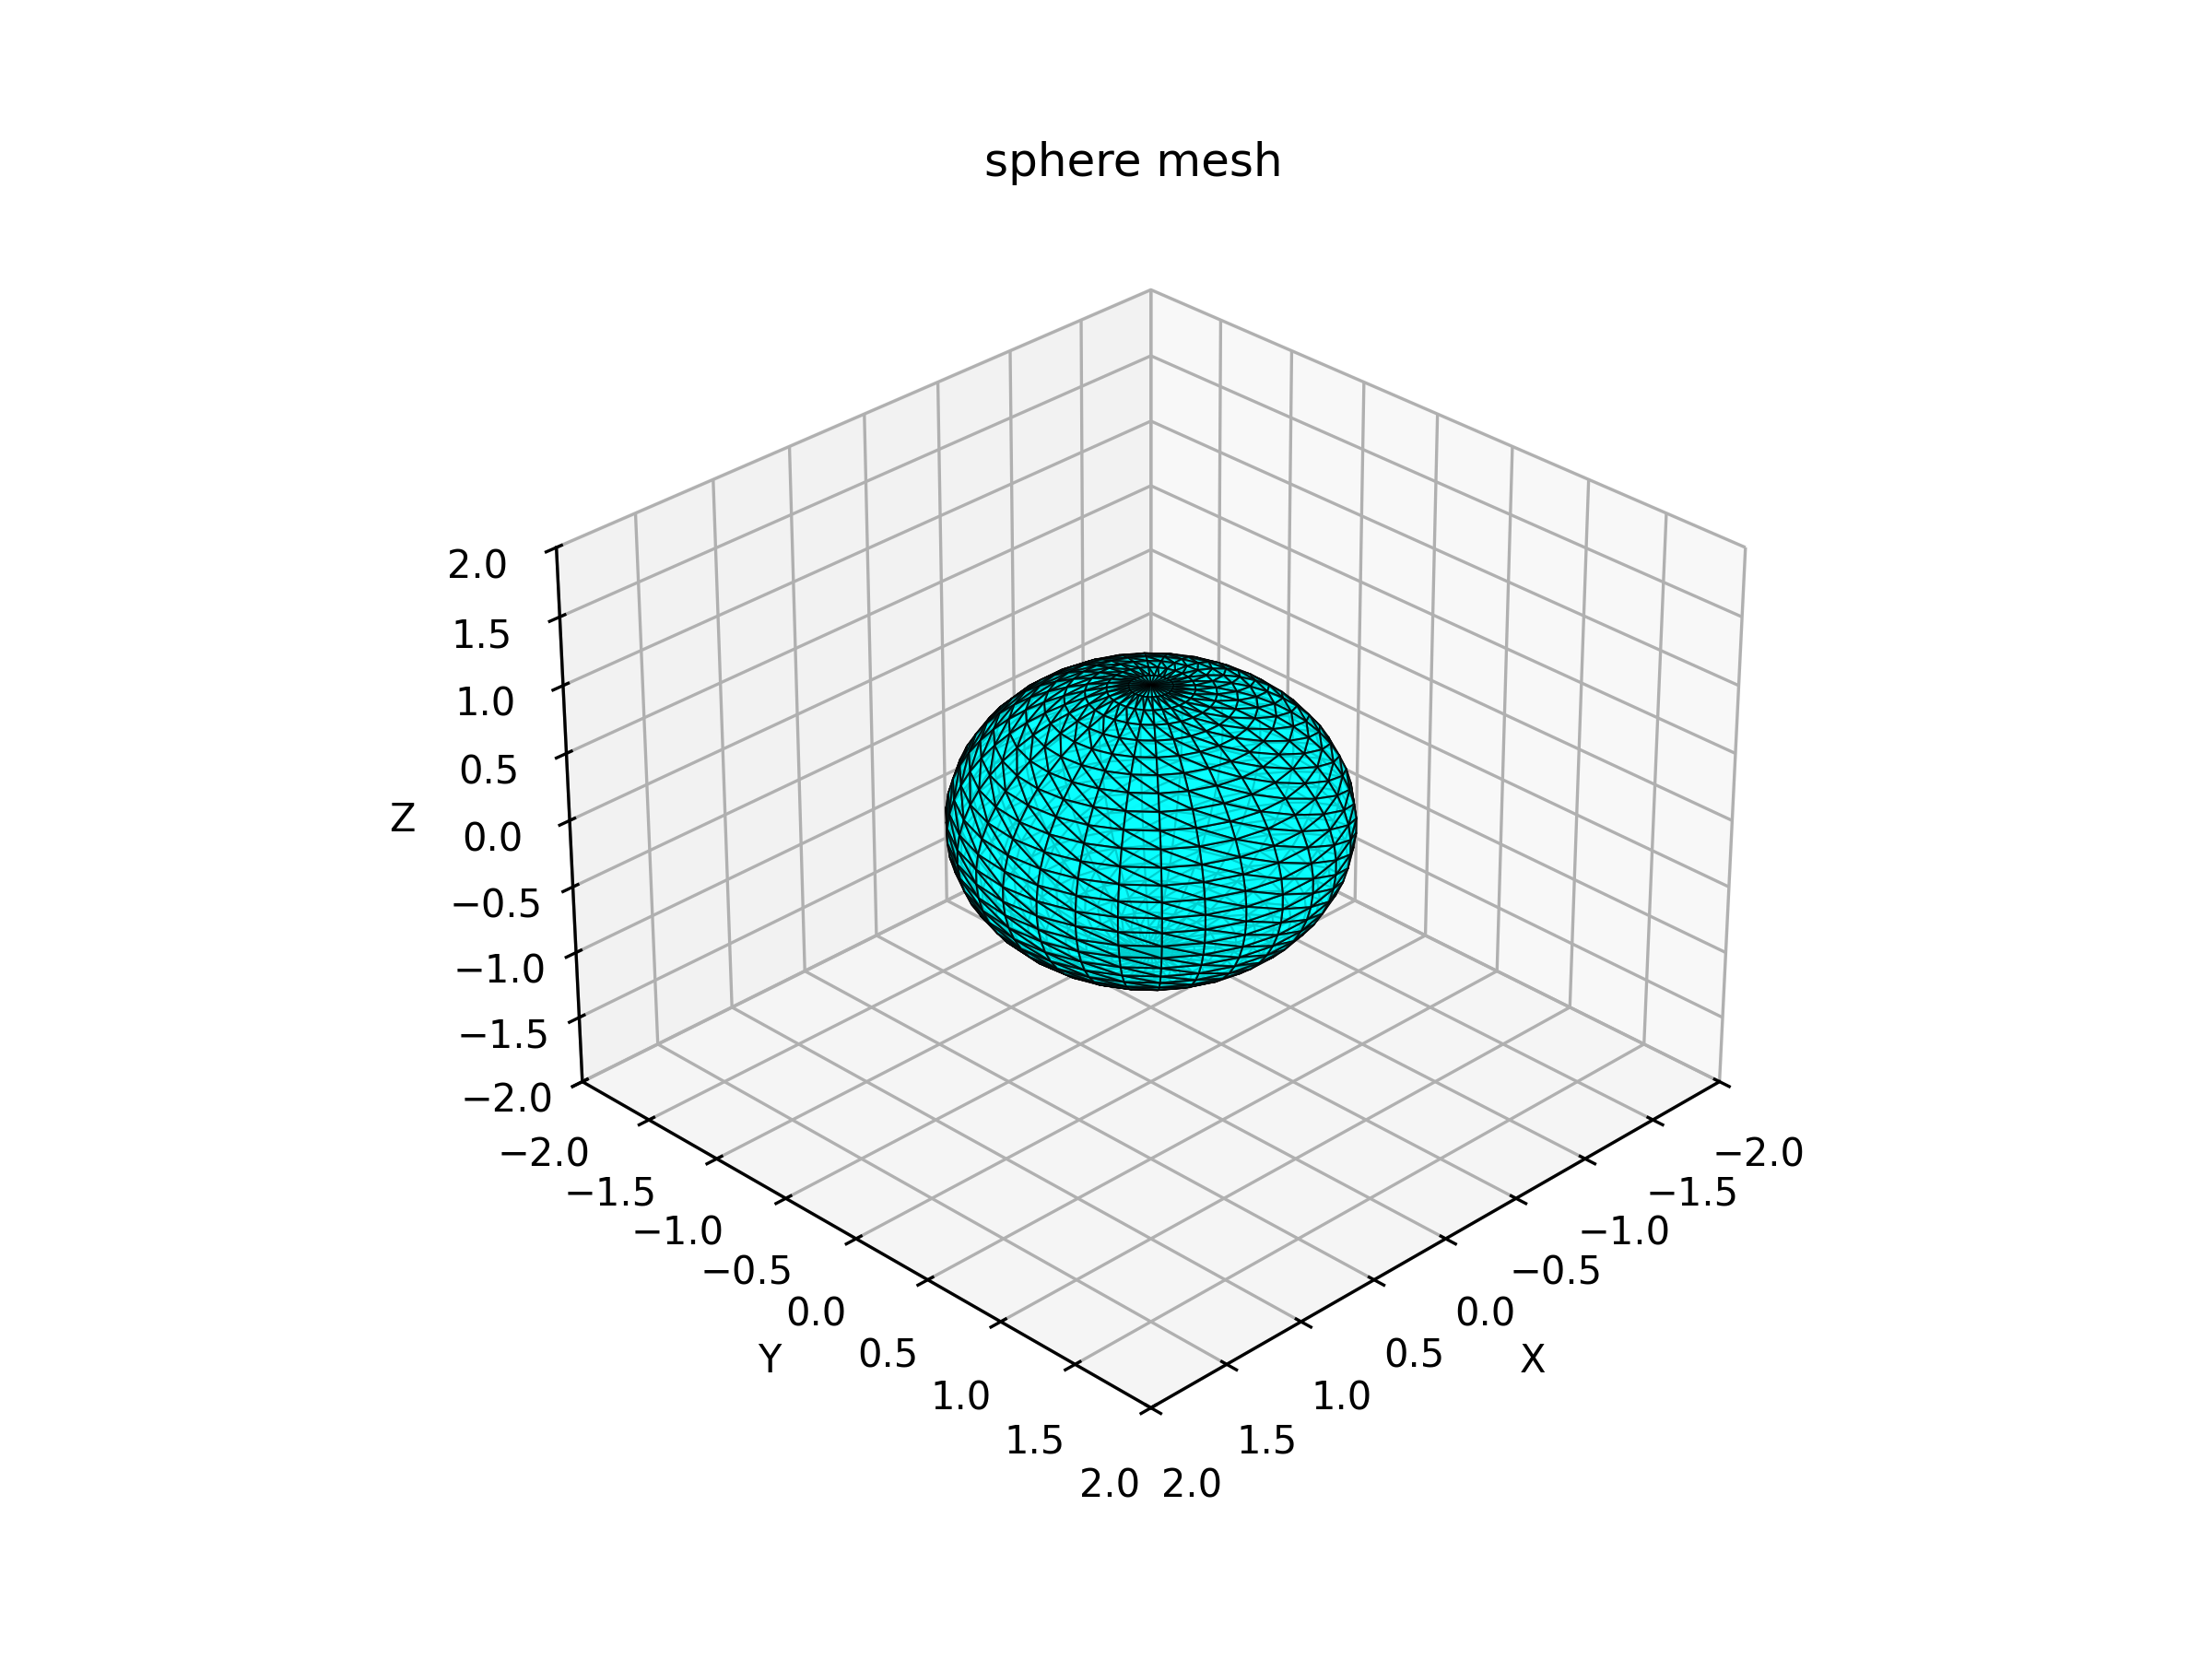
\includegraphics[width=1.1\linewidth]{../figs/sphere.png}

    \end{minipage}%
    \hfill
    \begin{minipage}{0.3\textwidth}
        \centering
        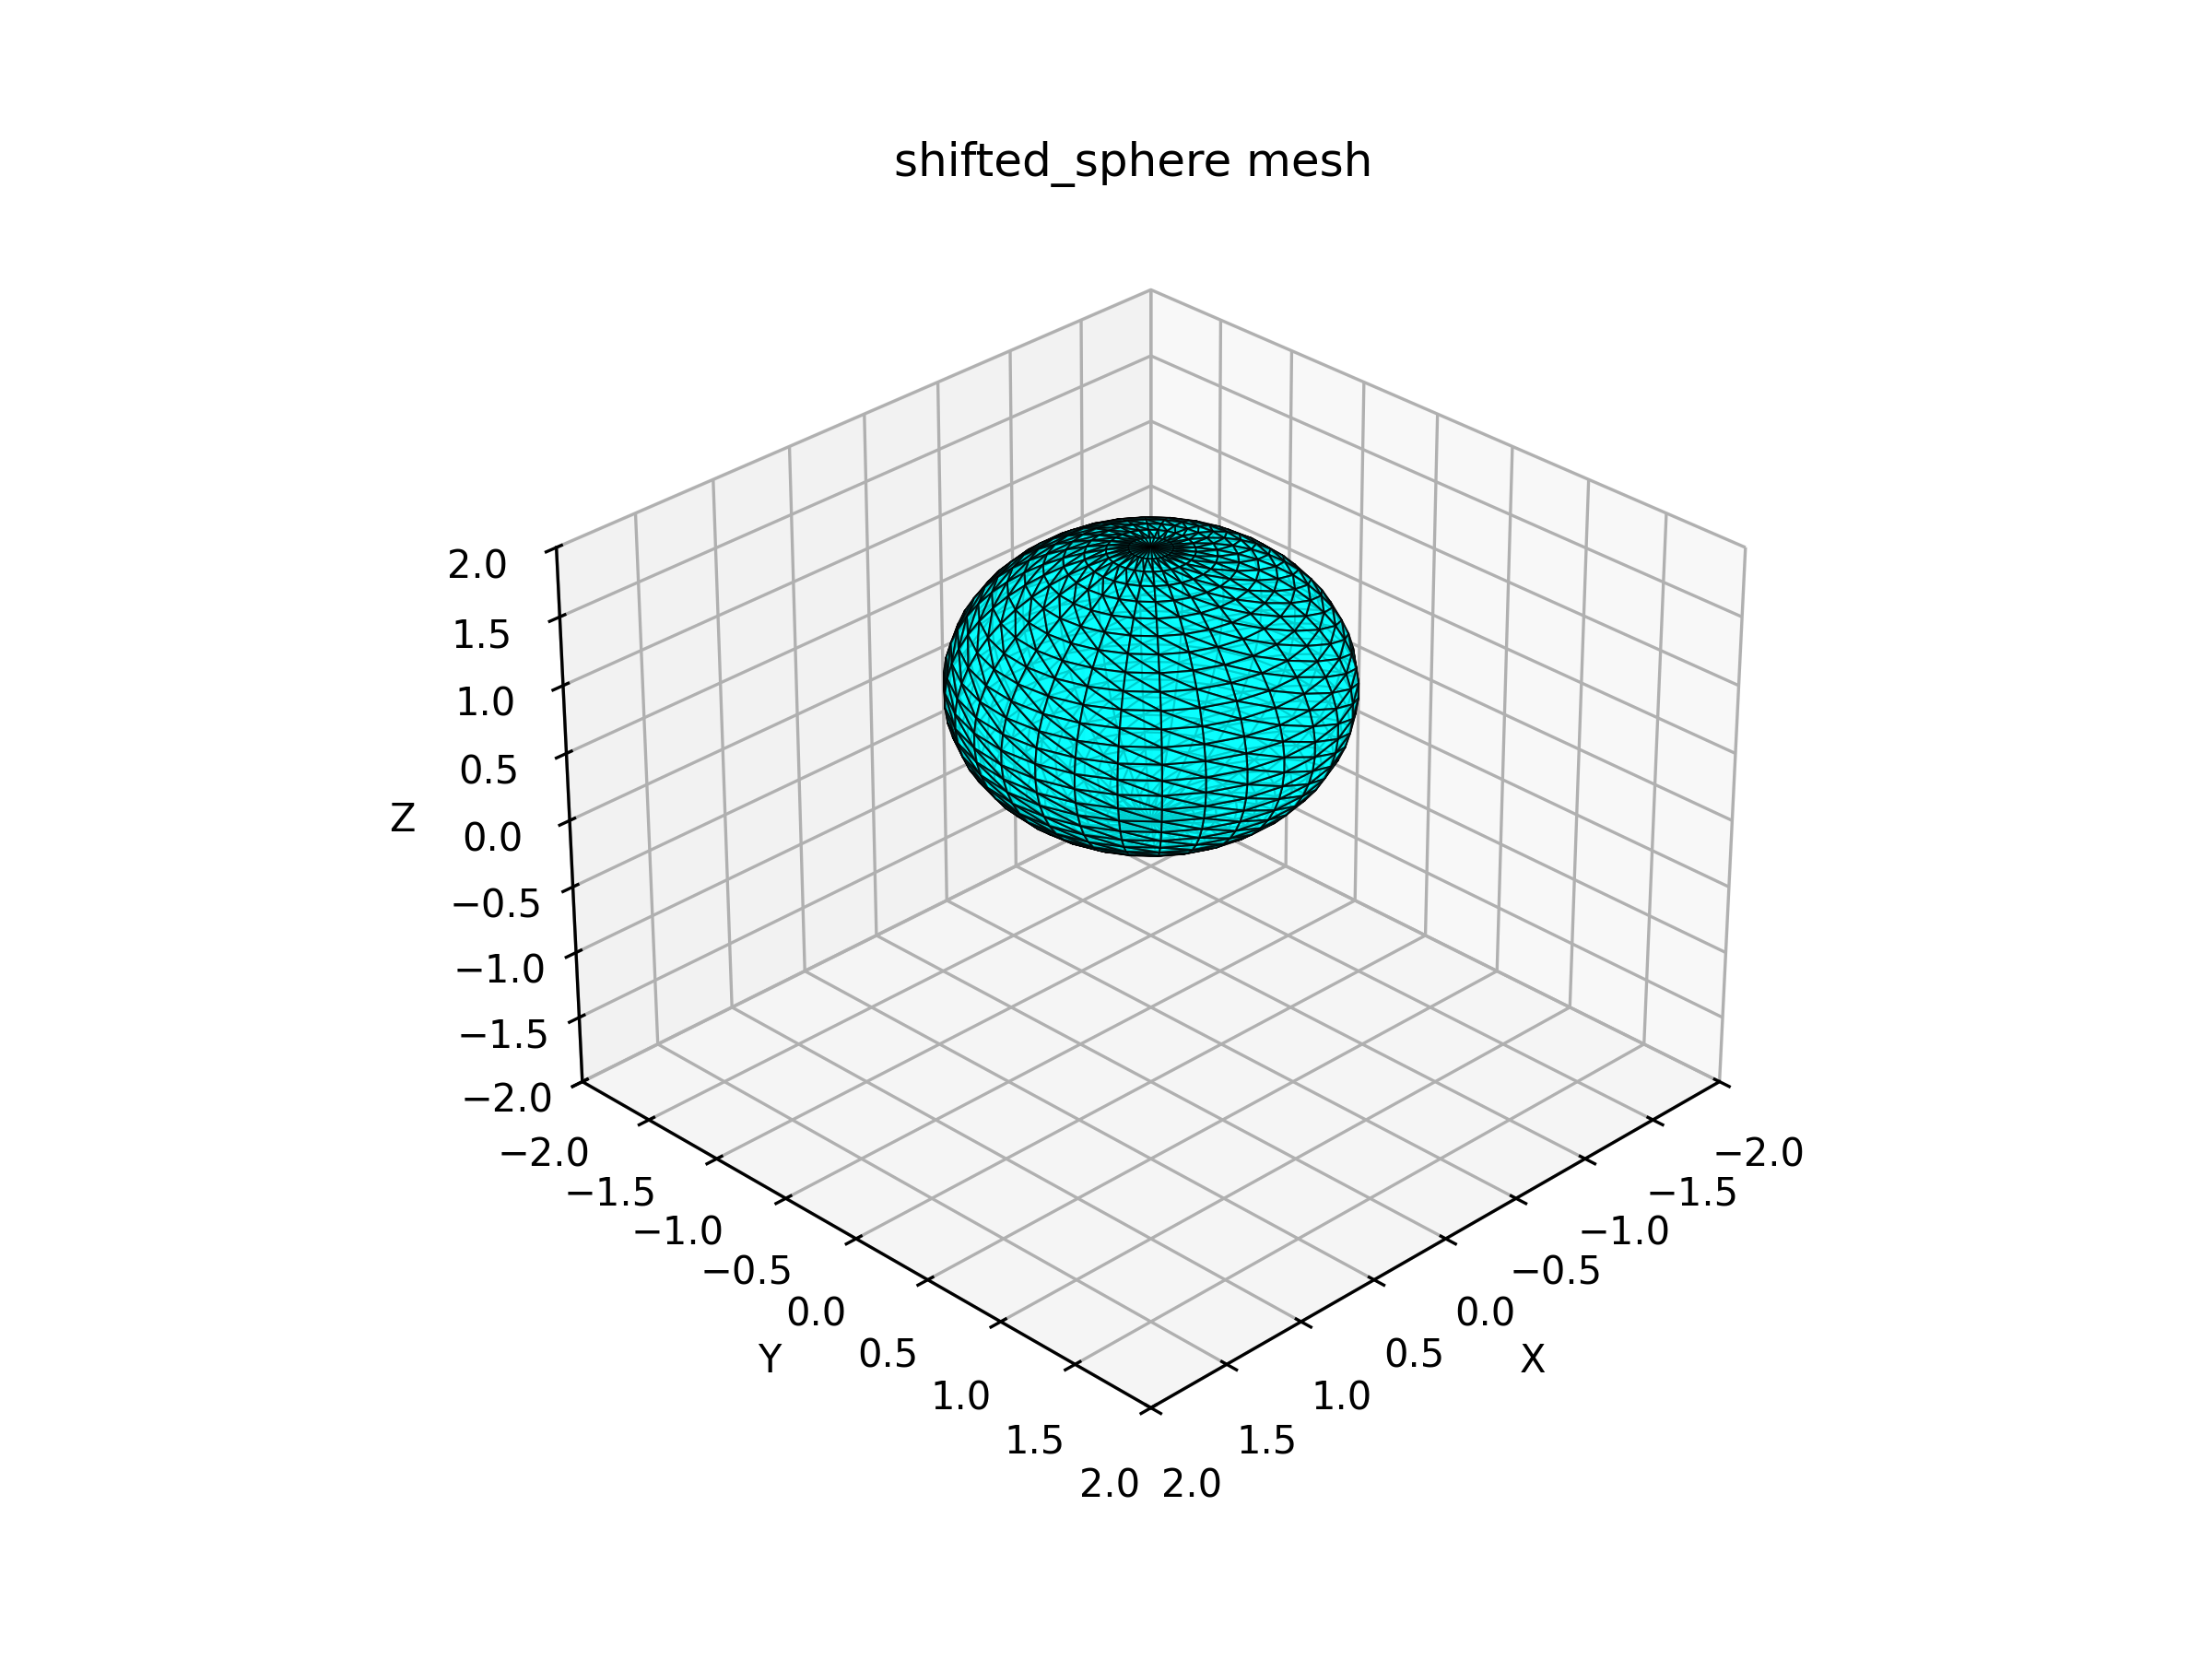
\includegraphics[width=1.1\linewidth]{../figs/shifted_sphere.png}

    \end{minipage}%
    \hfill
    \begin{minipage}{0.3\textwidth}
        \centering
        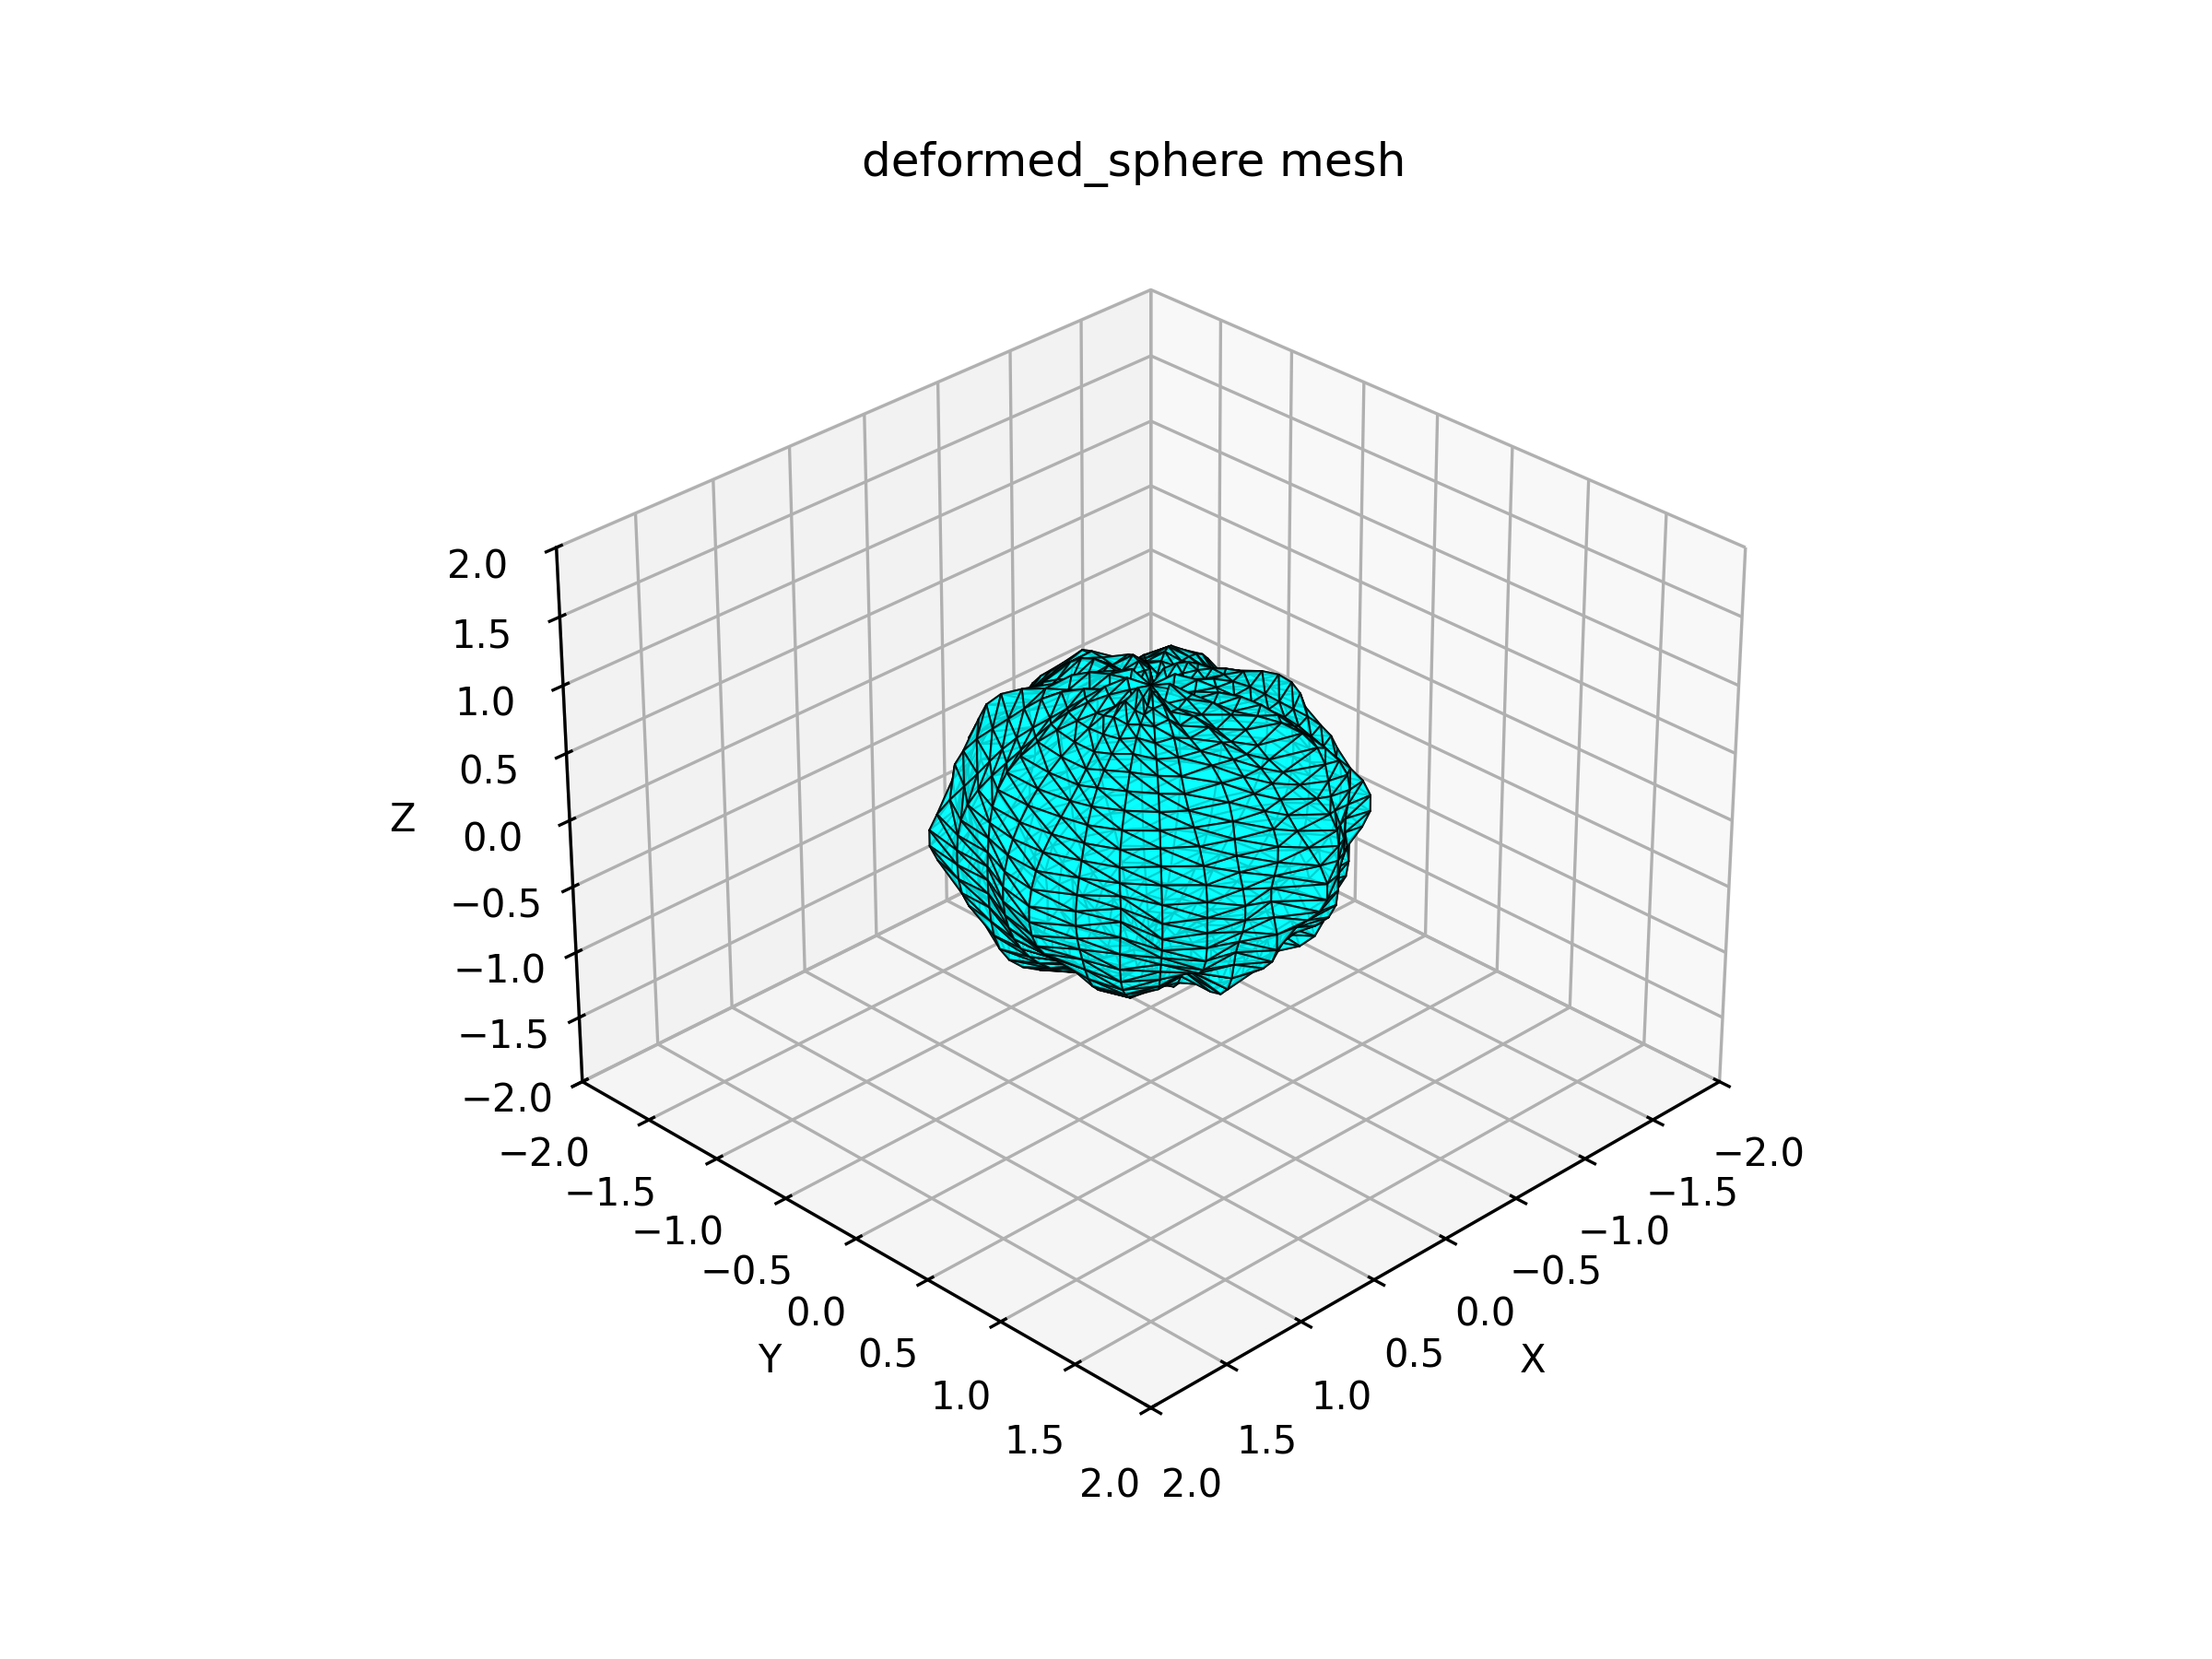
\includegraphics[width=1.1\linewidth]{../figs/deformed_sphere.png}

    \end{minipage} \\
    \vspace{0.5cm} % Adds some vertical space between rows

    \begin{minipage}{0.3\textwidth}
        \centering
        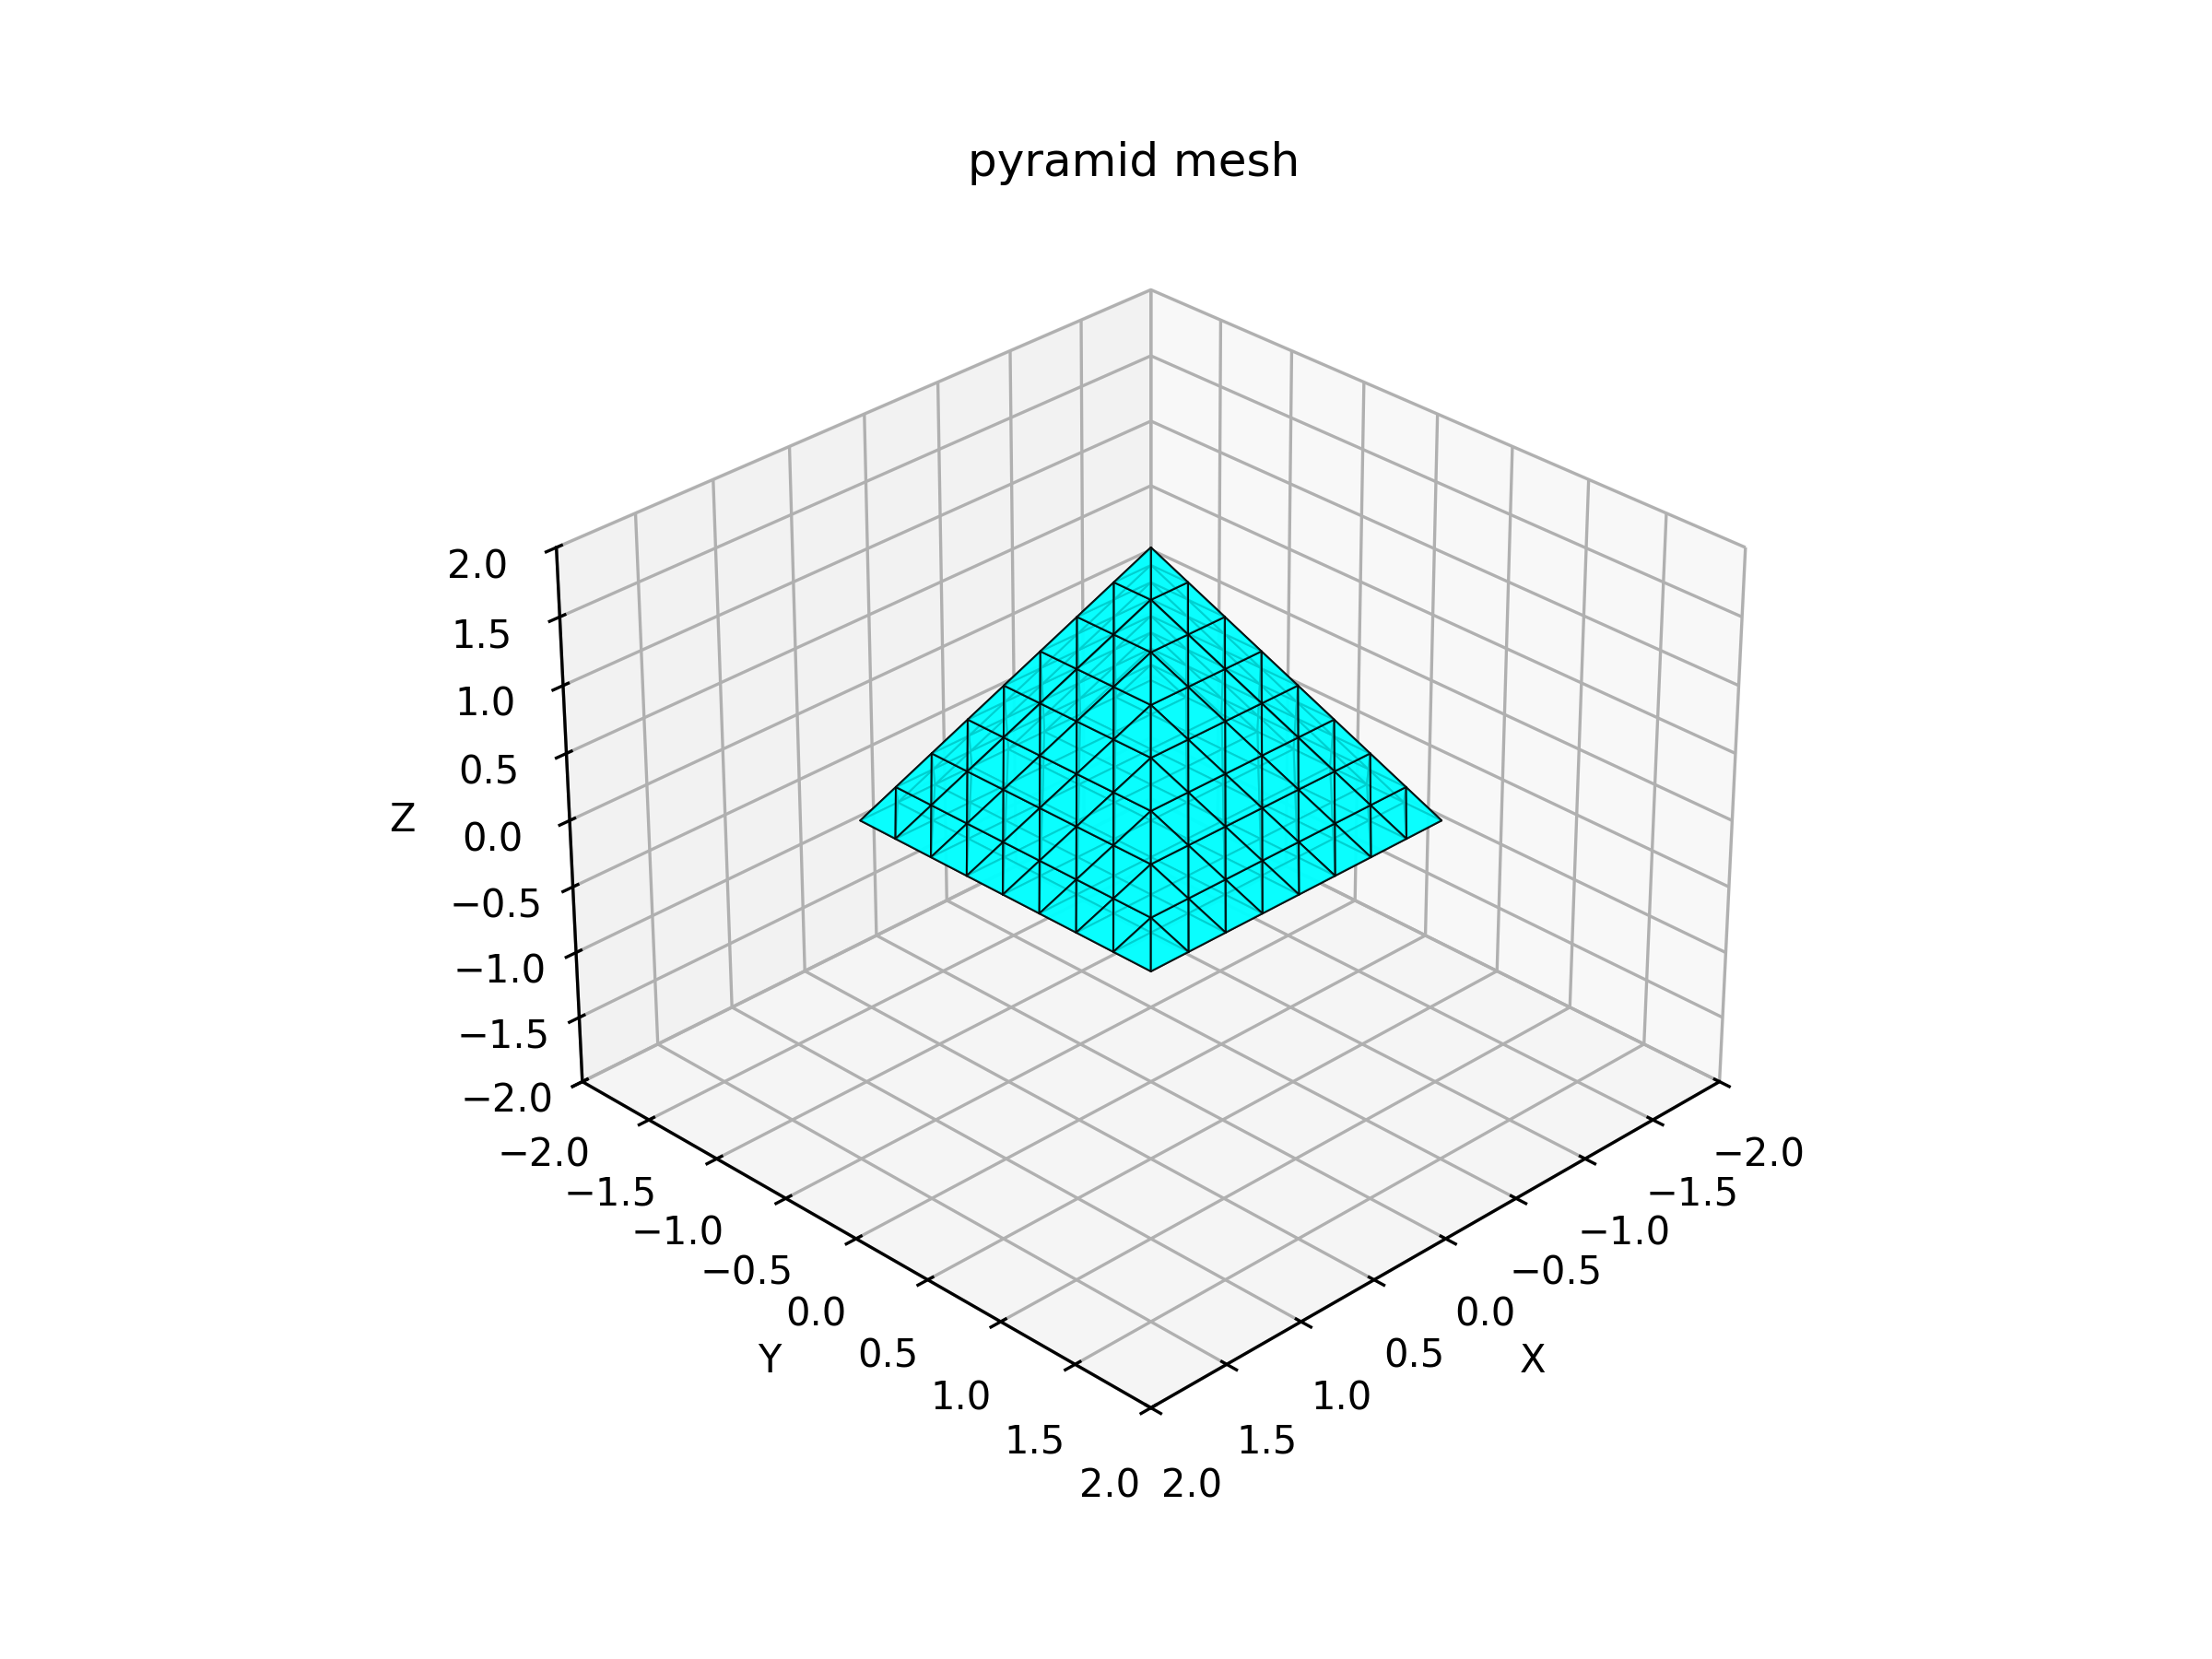
\includegraphics[width=1.1\linewidth]{../figs/pyramid.png}

    \end{minipage}%
    \hfill
    \begin{minipage}{0.3\textwidth}
        \centering
        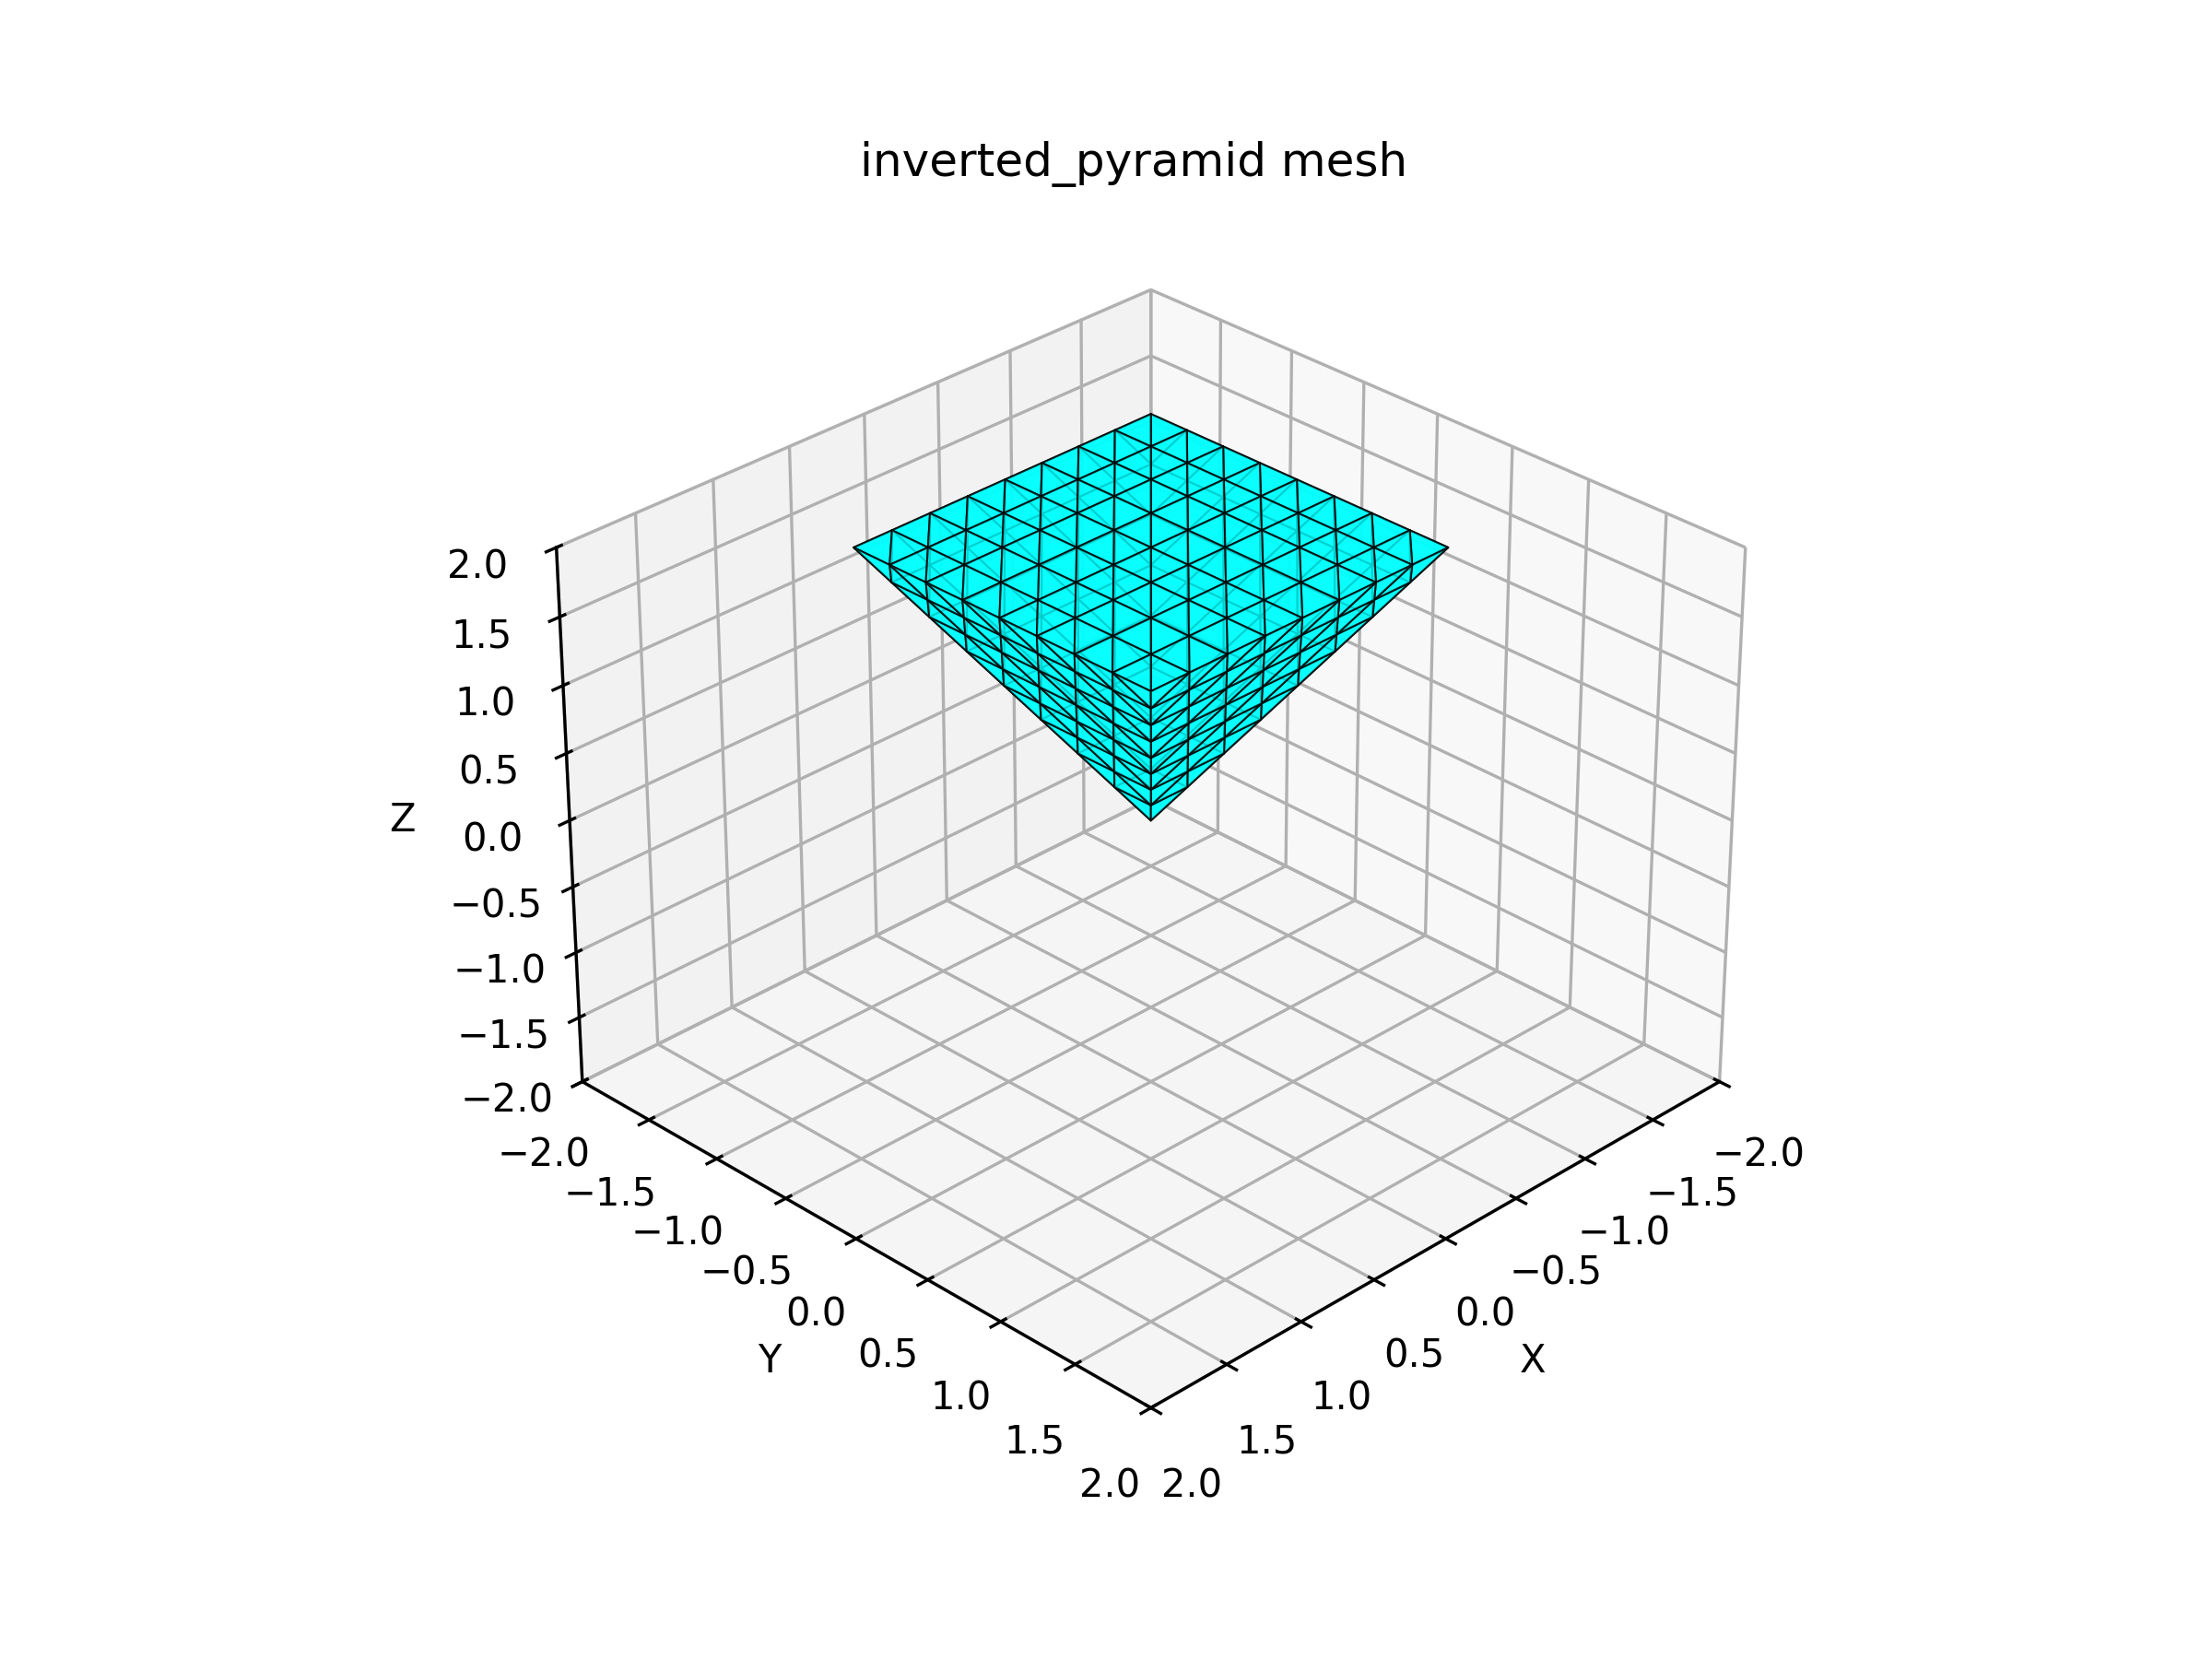
\includegraphics[width=1.1\linewidth]{../figs/inverted_pyramid.png}

    \end{minipage}%
    \hfill
    \begin{minipage}{0.3\textwidth}
        \centering
        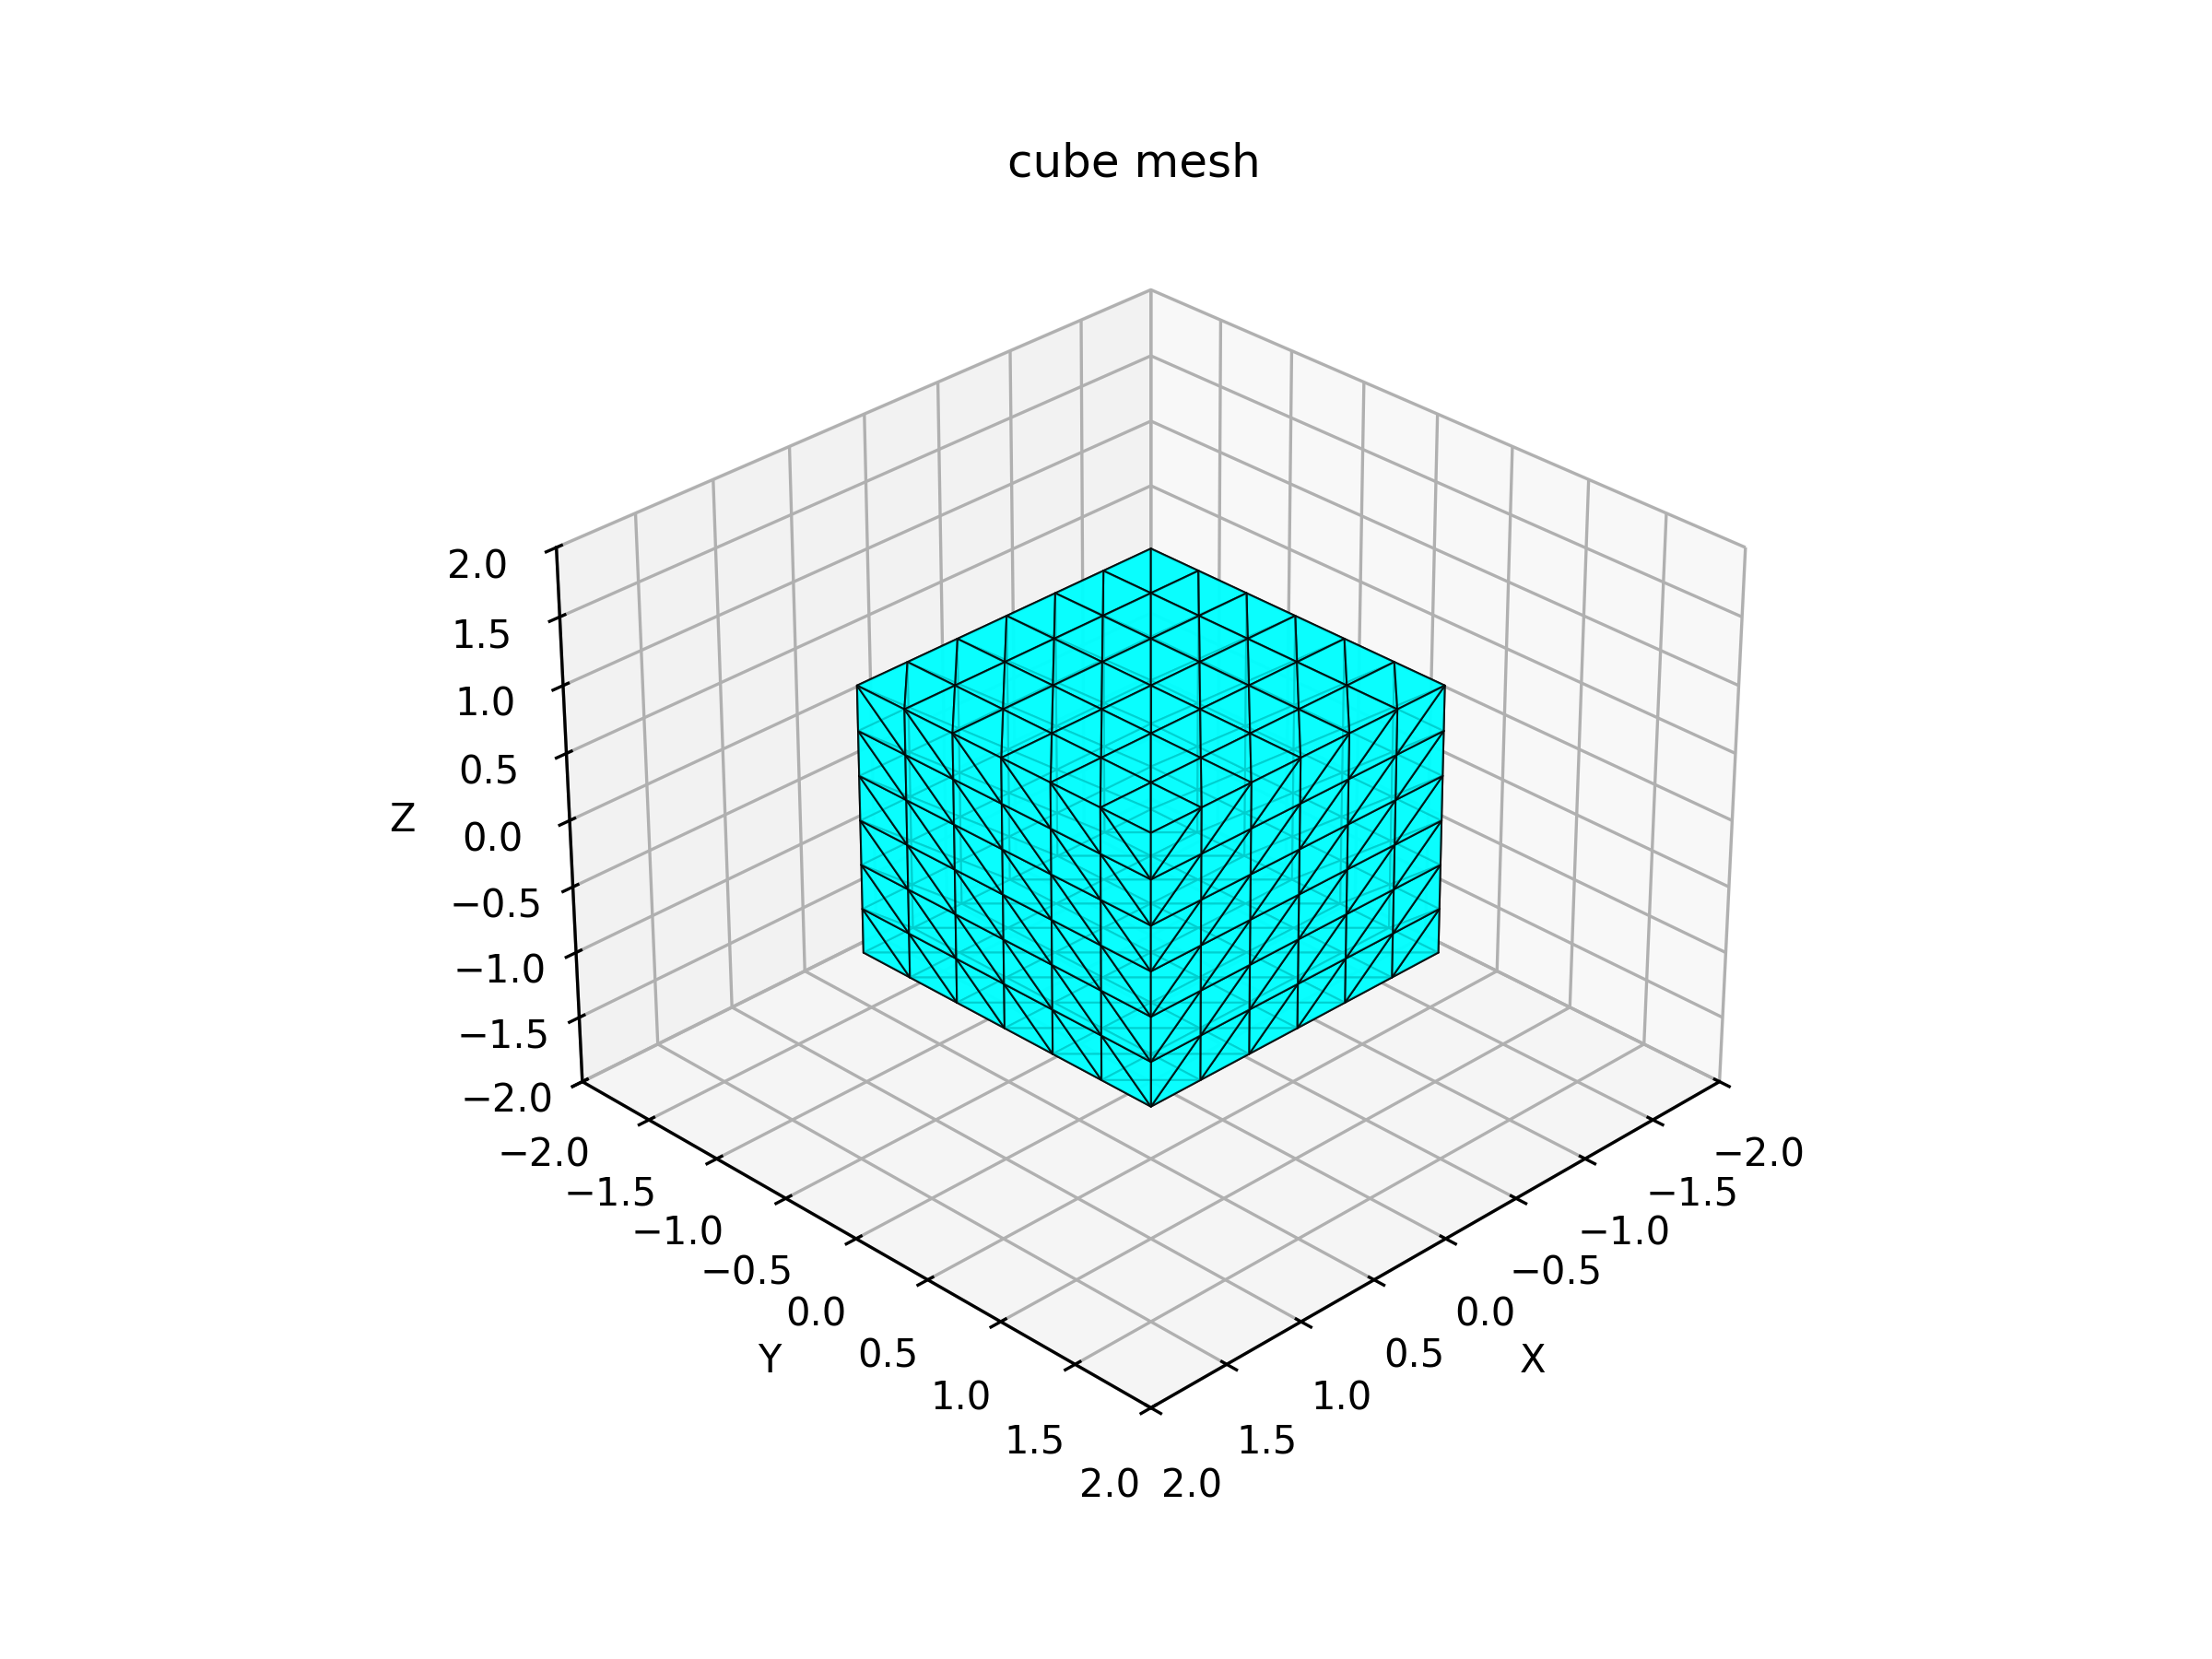
\includegraphics[width=1.1\linewidth]{../figs/cube.png}

    \end{minipage} \\
    \vspace{0.5cm}

    \begin{minipage}{0.3\textwidth}
        \centering
        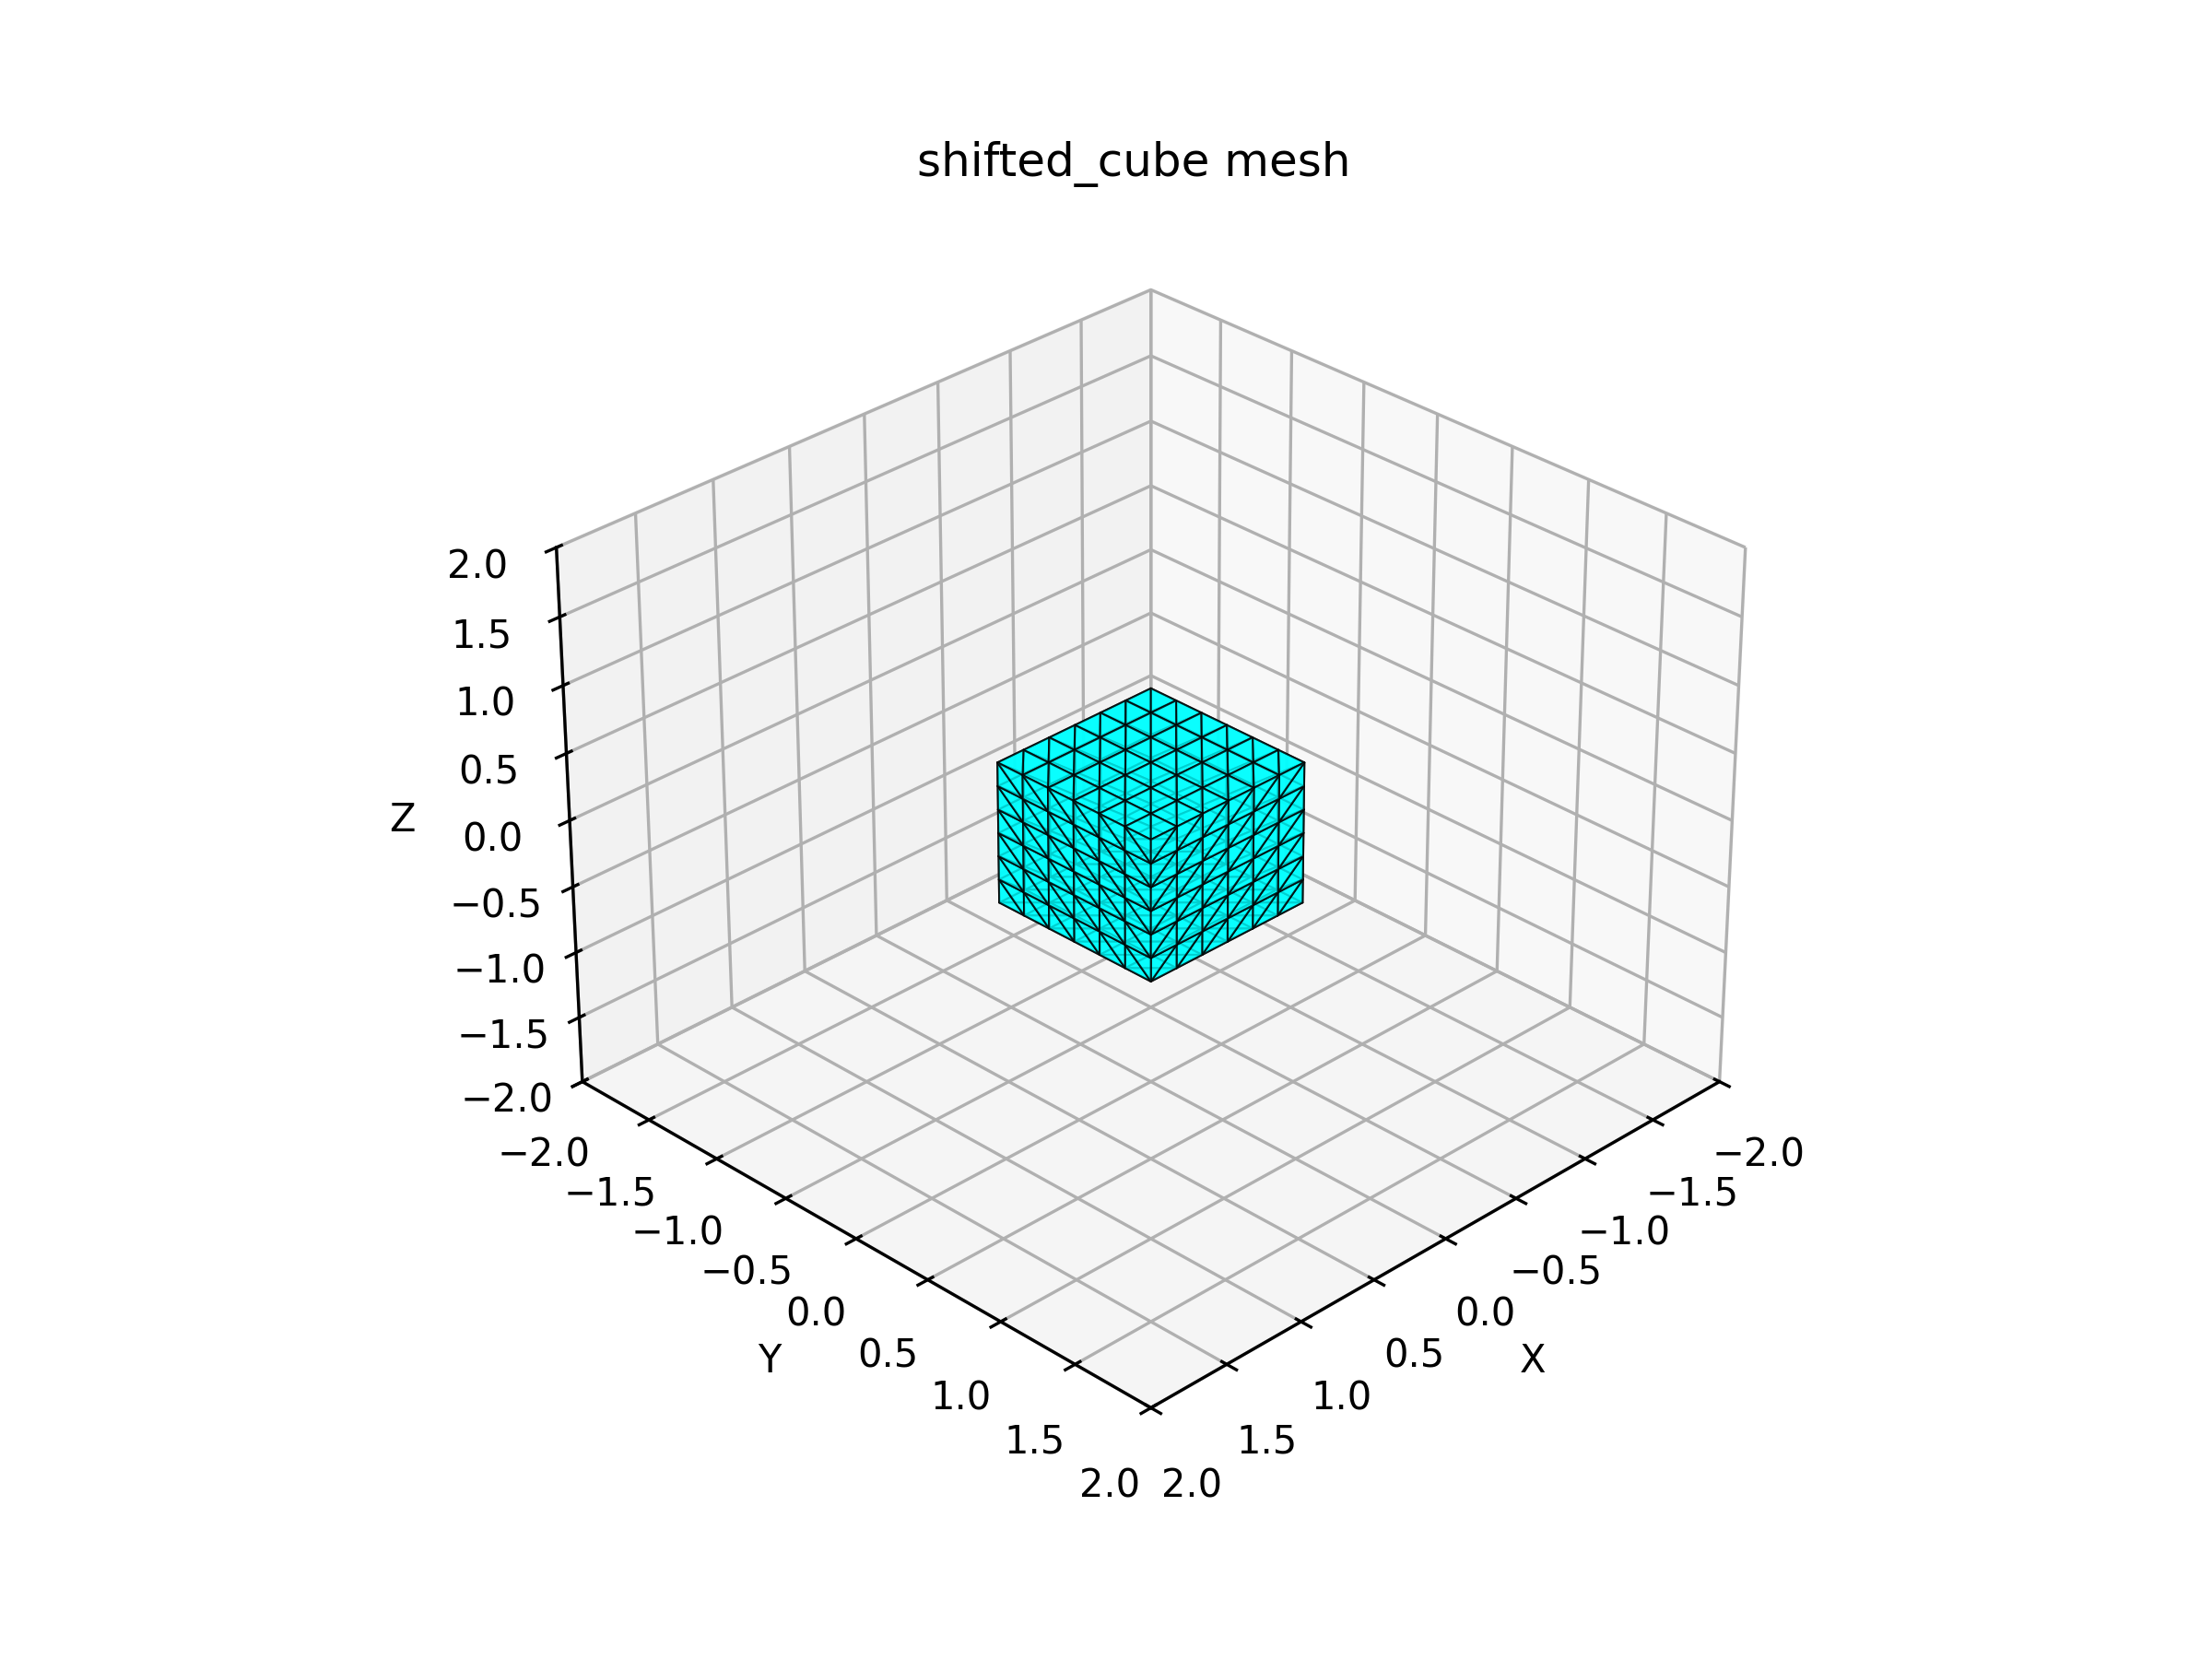
\includegraphics[width=1.1\linewidth]{../figs/shifted_cube.png}

    \end{minipage}

    \caption{Some shapes.}
    \label{fig:all_figures}
\end{figure}

The shapes presented in Figure \ref{fig:all_figures} are a sphere, a translated sphere, a deformed sphere, a pyramid, an inverted pyramid, a cube and a translatedi and scaled down cube. We then compute the Hausdorff distance and the Euclidean distance between the Eigenvalues for all pair combinations. The results of this calculation are presented in the following distance matrices:

\begin{figure}[H]
    \centering
    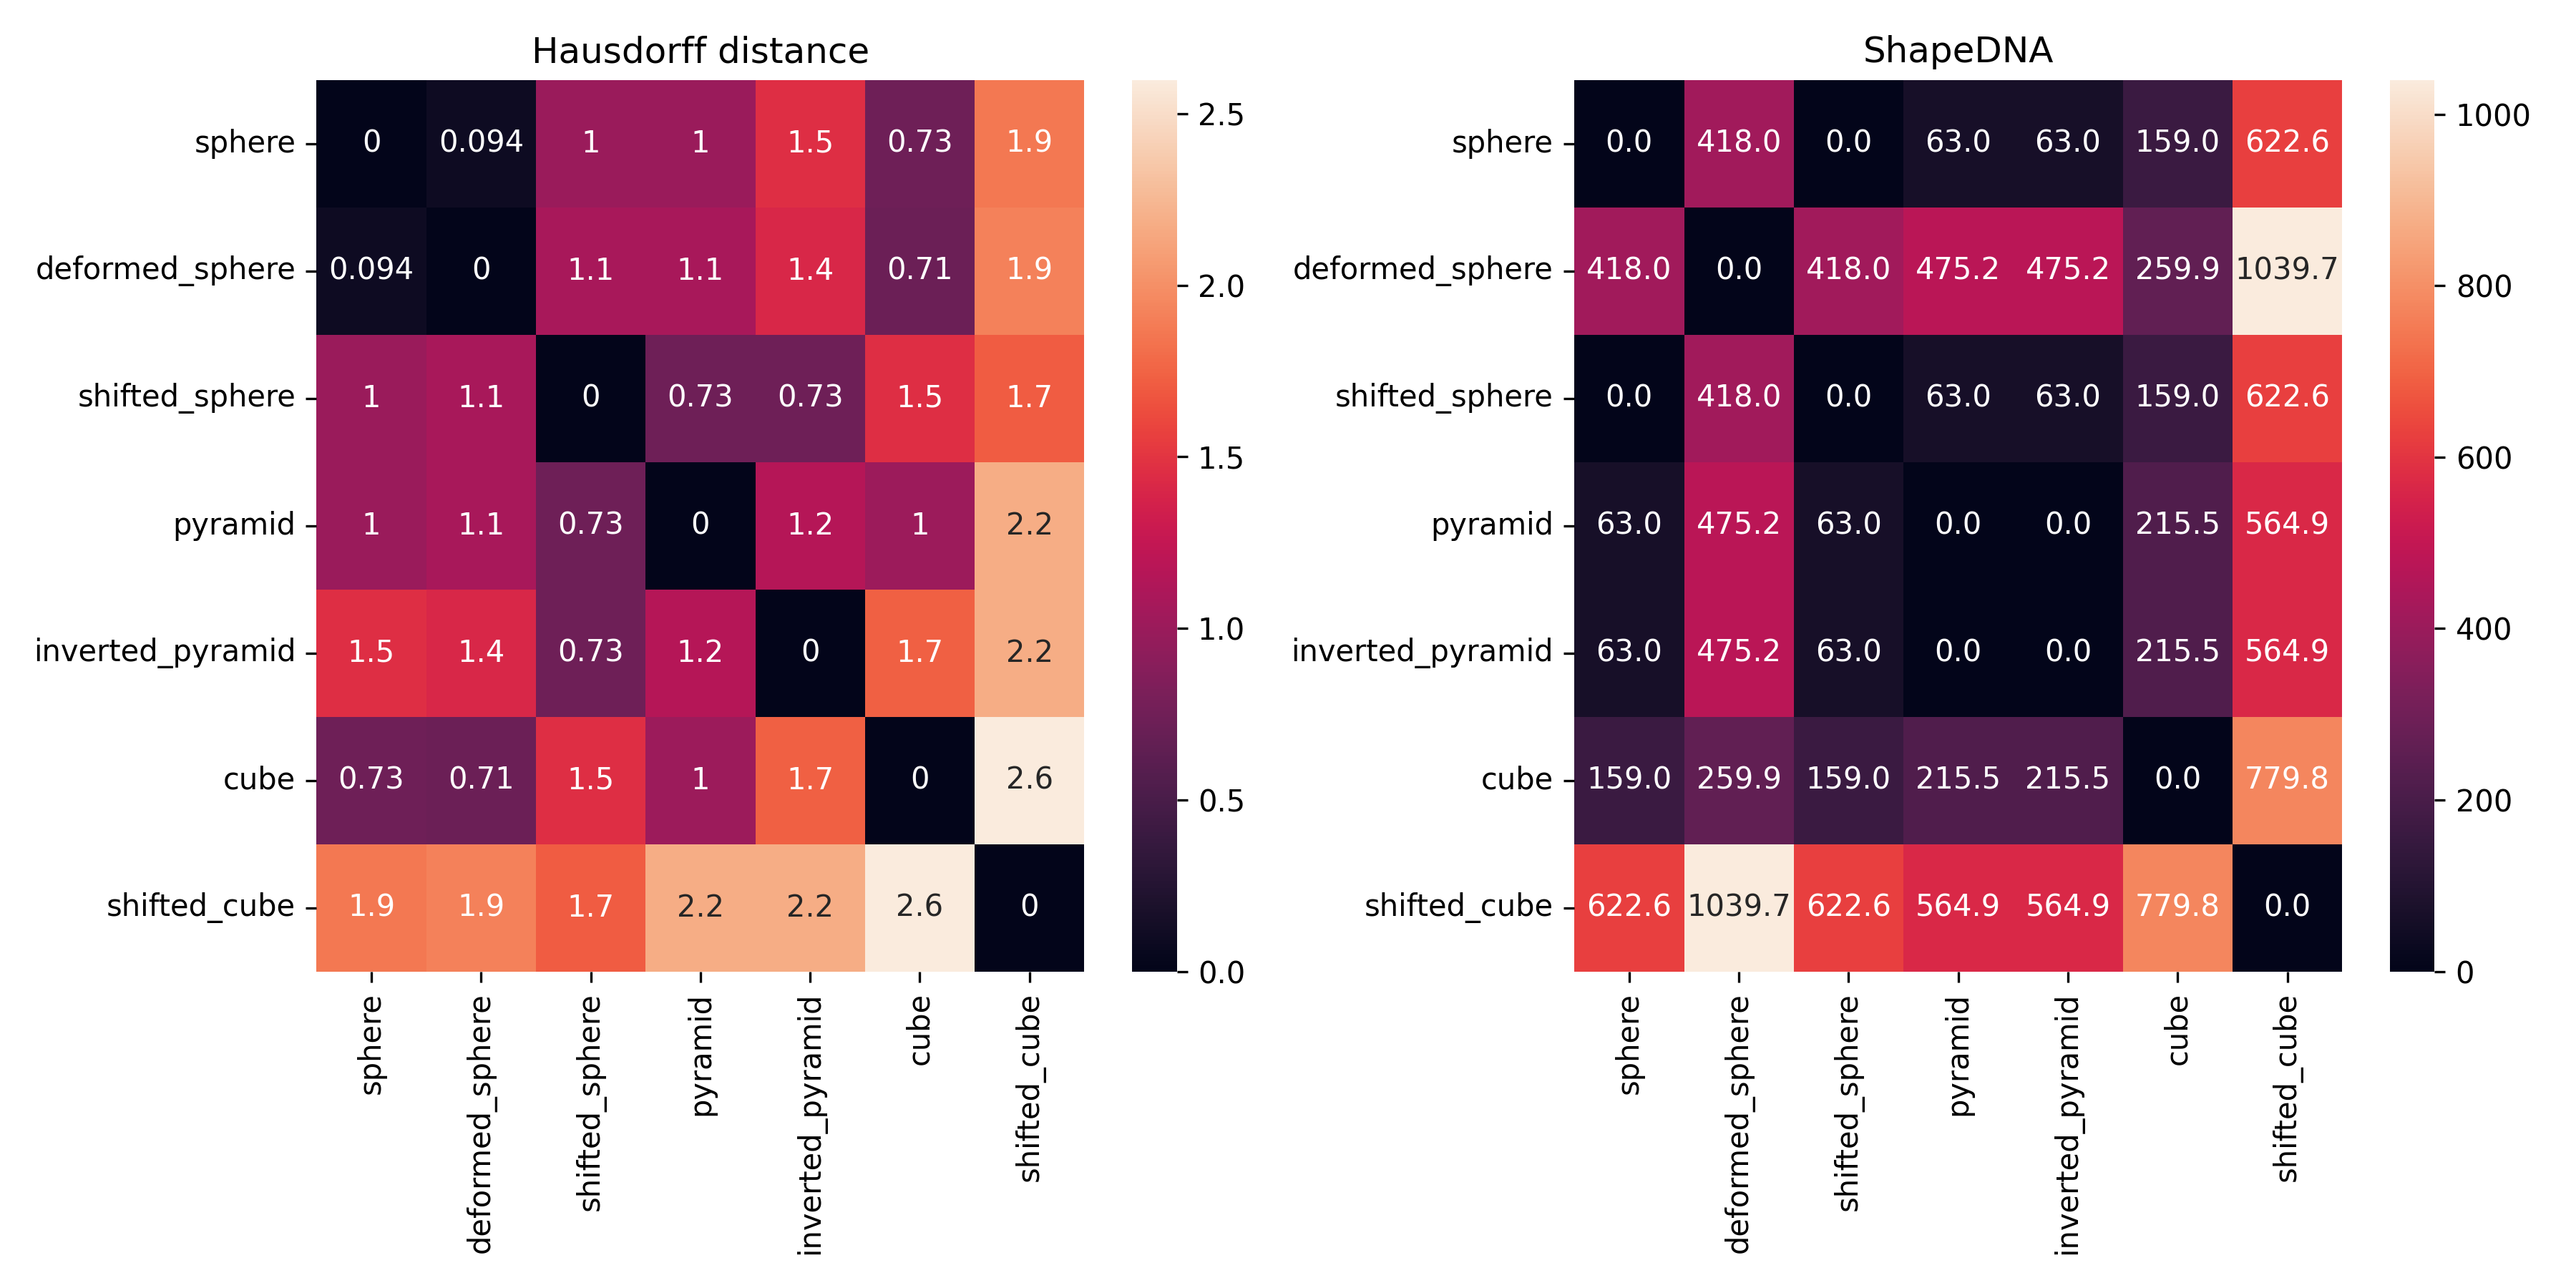
\includegraphics[width=\linewidth]{../figs/results/distance_matrices.png}  % Adjust the width or scale as needed
    \caption{Left: Hausdorff distance matrix. Right: Euclidean distance between Laplace-Beltrami Eigenvalues distance matrix.}
    \label{fig:d_matr}
\end{figure}

We can see in Figure \ref{fig:d_matr} that the Hausdorff metric fails to take into account translation and rotation (see sphere vs shifted sphere and pyramid vs inverted pyramid). For example, distance between a sphere and a shifted sphere is the same as that between a sphere and a pyramid, and interestingely even greater between a sphere and an inverted pyramid. More notably, the the Hausdorff distance between the sphere and the deformed sphere is small - this is because most of the deformation information is encoded in the connectivity of the mesh, rather than the point cloud data. \par

As for the ShapeDNA method, the deformed sphere exhibits the largest distance to all other objects. As expected, the translated and rotated objects have the same Eigenvalues (and hence Euclidean distance of zero) - in particular the sphere and the shifted sphere and pyramid and the inverted pyramid. Interestingely, the deformed sphere is least similar to the shifted and scaled down cube and most similar to the zero-cented unit cube. Here we have used $75$ Eigenvalues of the Laplace-Beltrami operator; it is important to point out that Euclidean distance may not be the best choice of a distance metric due to the high dimensionality; other strategies for comparing the spectra are discussed in the original paper \cite{shapedna}. Nevertheless, we still obtain intuitive and interpretable results. To understand the behaviour of this metric better, we next shift our attentiont to the entire dataset.

\begin{figure}[H]
    \centering
    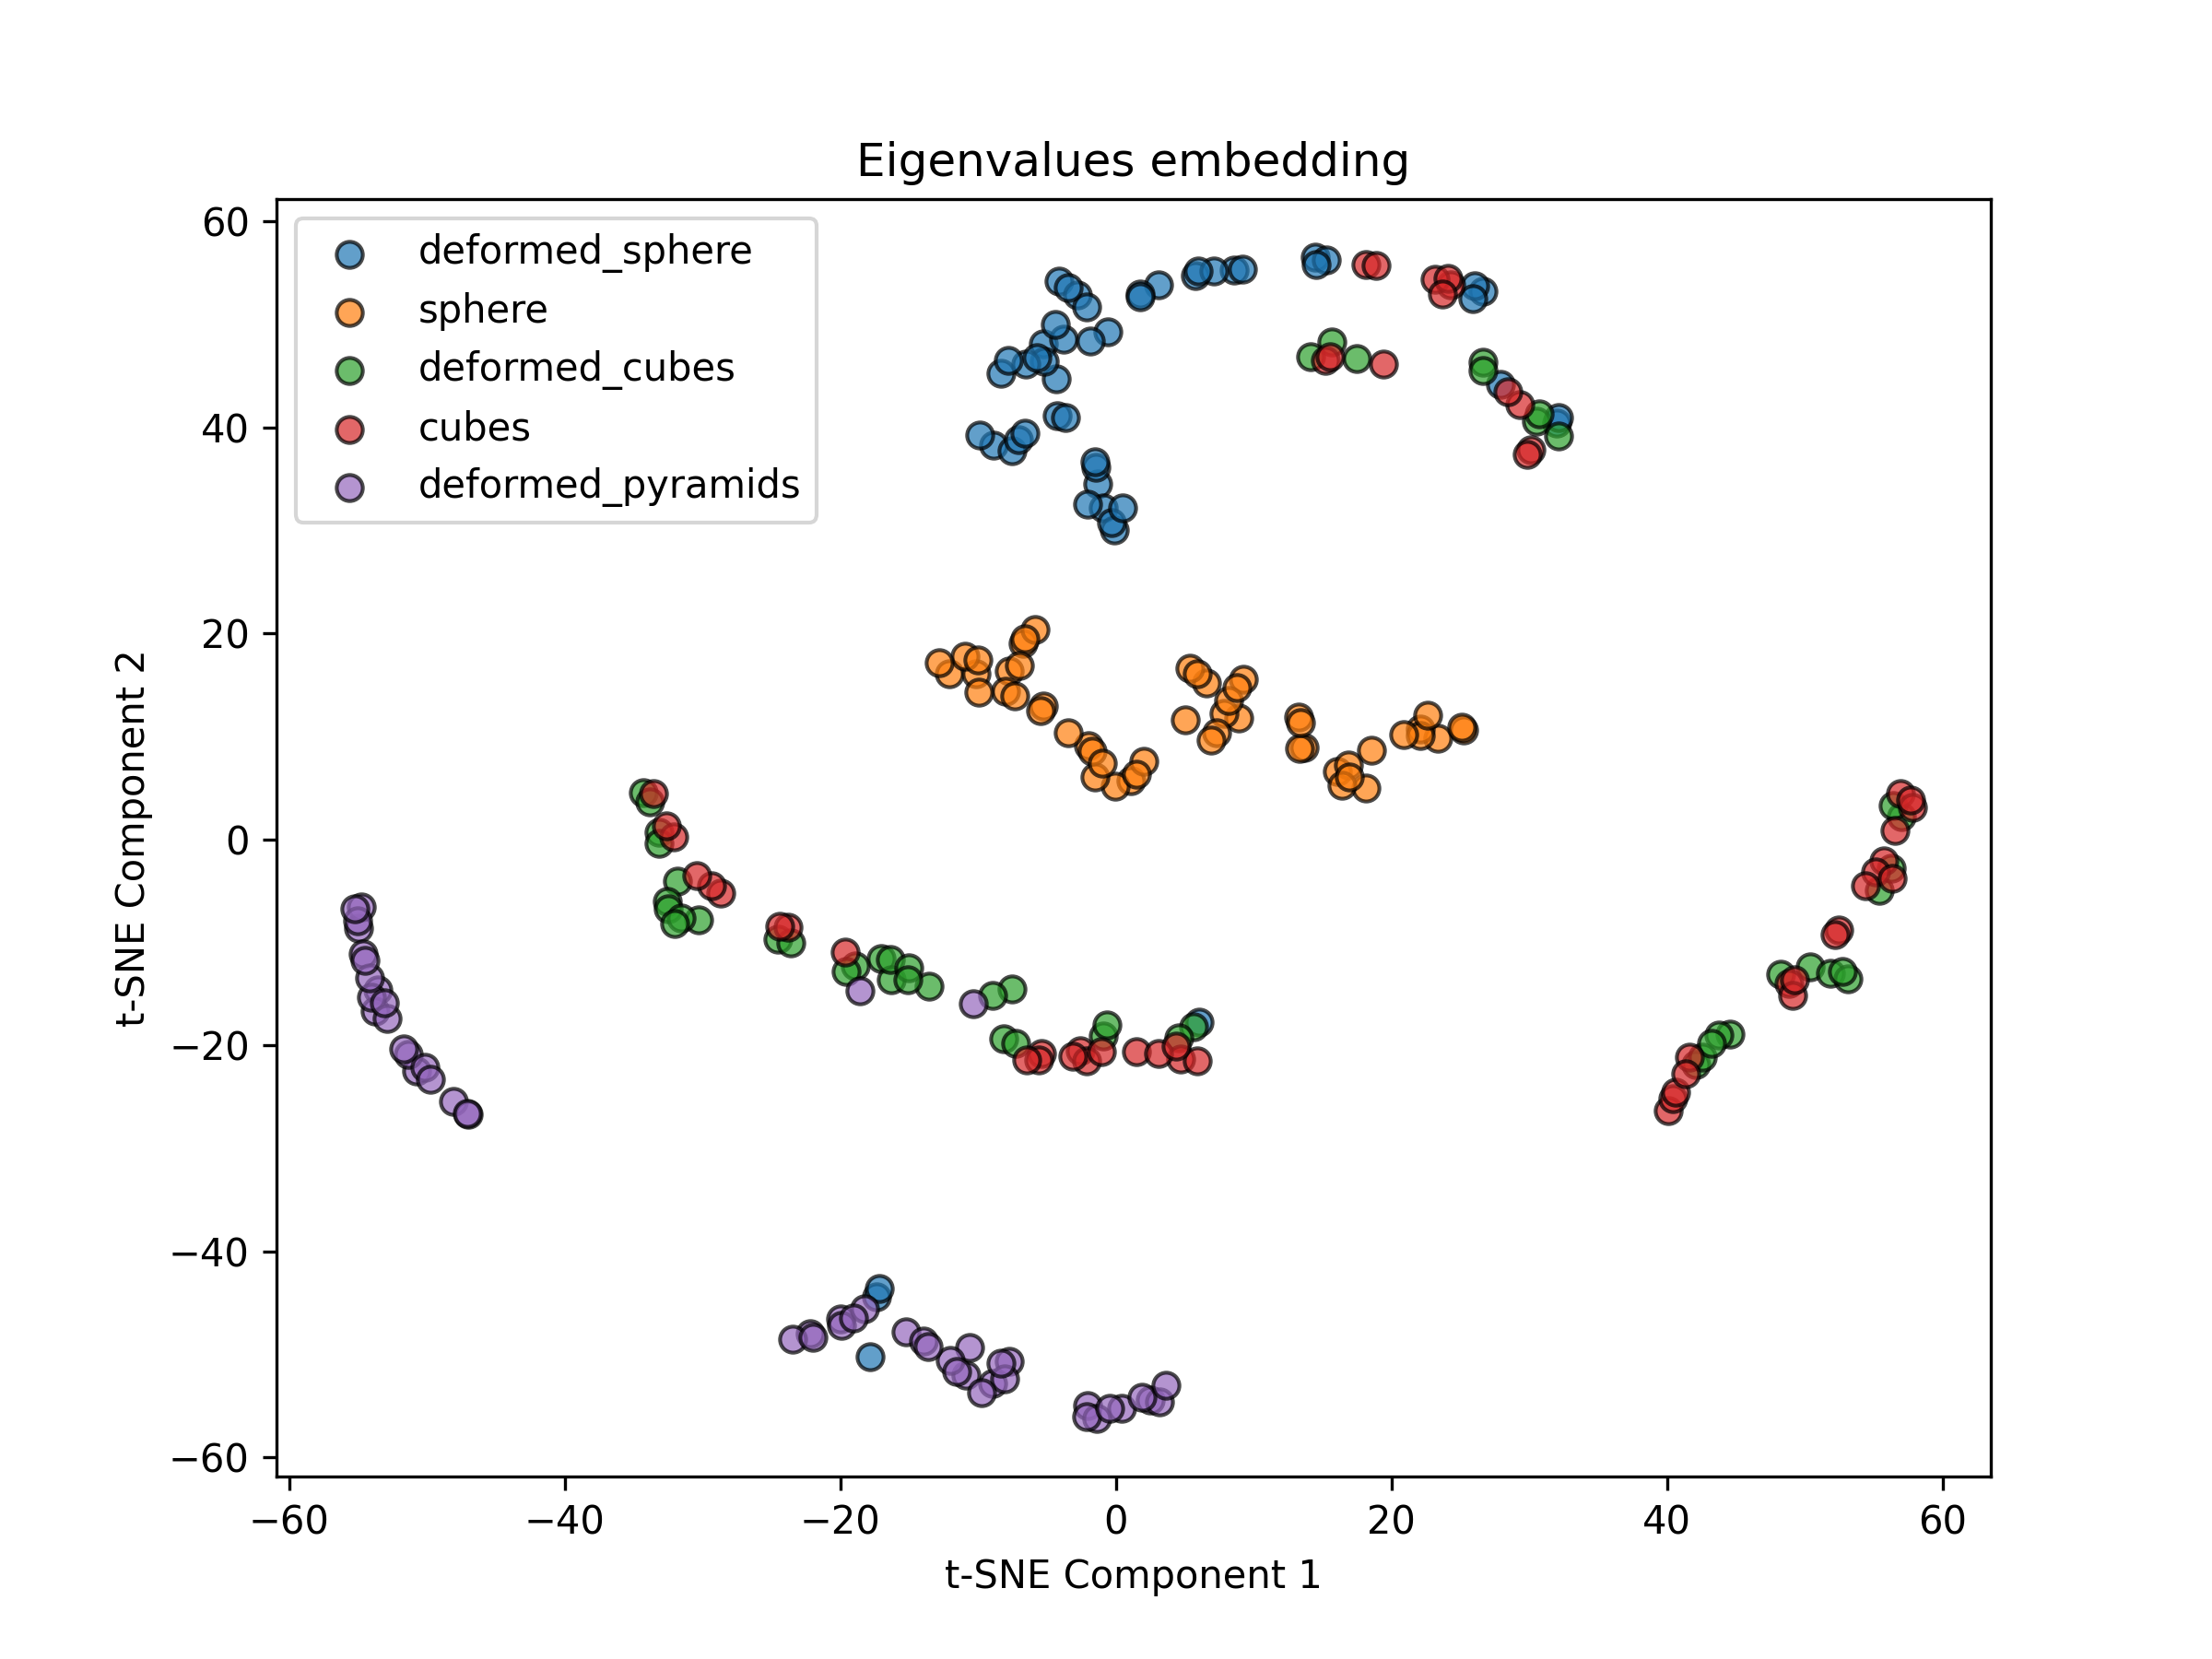
\includegraphics[width=\linewidth]{../figs/results/tsne_embedding.png}  % Adjust the width or scale as needed
    \caption{tSNE embedding of all 255 shape Eigenvalues.}
    \label{fig:tsne}
\end{figure}

The embedding in Figure \ref{fig:tsne} reveals that the ShapeDNA method successfully captures the similarity and differences between the five groups we used in this case study. The deformed pyramids segment nicely from the other groups. Cubes and deformed cubes overlap - it would be interesting to see what would happen if we increased the level of deformation. In contrast to this, spheres and deformed spheres seem to be separated in the embedding space, with some cubes and deformed cubes sneaking into the deformed spheres category. This result reveals that the Laplace-Beltrami Eigenvalues spectrum successfully captures the differences and similarities between our simple geometrical shapes. Here we use $75$ Eigenvalues for each object, so it would be interesting what a optimal number of Eigenvalues to use would be.

\section{Conclusions}
We successfully implemented and tested a popular method for comparing 3D meshes. With the aid of dimensionality reduction we can see that the Eigenvalues spectrum holds valuable information about the spatial structure of such meshes. The Eigenvalues can also potentially be used as an input to a neural network. Another interesting approach for comparing shapes, which is not discussed here is with the use of the hyperbolic Wasserstein distance \cite{hyp_w}. 

\printbibliography

\end{document}
